\documentclass[11pt]{article}

\usepackage{fullpage}
\usepackage{rotating}   
\usepackage{amsmath}
\usepackage{amssymb}
\usepackage{amsthm}
\usepackage{fancyhdr}
\usepackage{algorithm}
\usepackage{algorithmic}
\usepackage{bm}
\usepackage{listings}
\usepackage{graphicx}
\usepackage{caption2}
\usepackage{subfigure}
\usepackage{float}
\usepackage{extpfeil}
\usepackage{color}
\usepackage[usenames,dvipsnames]{xcolor}


\newtheorem{theorem}{Theorem}[section]
\newtheorem{lemma}[theorem]{Lemma}
\newtheorem{corollary}[theorem]{Corollary}
\newtheorem{proposition}[theorem]{Proposition}
\newtheorem{definition}[theorem]{Definition}
\newtheorem{conjecture}[theorem]{Conjecture}
\newtheorem{remark}[subsection]{Remark}

%%
\newcommand\numberthis{\addtocounter{equation}{1}\tag{\theequation}}

%% define new symbols
\def\bx{\bm{x}}
\def\bb{\bm{b}}
\def\ba{\bm{a}}
\def\bc{\bm{c}}
\def\bf{\bm{f}}
\def\by{\bm{y}}
\def\bu{\bm{u}}
\def\bv{\bm{v}}
\def\BW{\bm{W}}
\def\BA{\bm{A}}
\def\bz{\bm{z}}
\def\BZ{\bm{Z}}
\def\BH{\bm{H}}
\def\BL{\bm{L}}
\def\BU{\bm{U}}
\def\BV{\bm{V}}
\def\BB{\bm{B}}
\def\BC{\bm{C}}
\def\BD{\bm{D}}
\def\BE{\bm{E}}
\def\BW{\bm{W}}
\def\BQ{\bm{Q}}
\def\BG{\bm{G}}
\def\BA{\bm{A}}
\def\BX{\bm{X}}
\def\BY{\bm{Y}}
\def\BQ{\bm{Q}}
\def\BI{\bm{I}}
\def\BR{\bm{R}}

%% define new brackets
\def\la{\left\langle}
\def\ra{\right\rangle}
\def\ln{\left\|}
\def\rn{\right\|}
\def\lb{\left(}
\def\rb{\right)}
\def\lsb{\left[}
\def\rsb{\right]}
\def\lcb{\left\{}
\def\rcb{\right\}}

%%
\DeclareMathOperator*{\argmin}{arg\,min}
\DeclareMathOperator*{\argmax}{arg\,max}

%%
\title{Homework XIV}
\author{Name: Shao Yanjun, Number: 19307110036}


\begin{document}
\maketitle

%------------------------------------
\begin{abstract}
This is Daniel's homework of  "Numerical Algorithms with Case Studies II".
\end{abstract}
%-------------------------------------
%=====================
\section{Problems}
\paragraph{Q1}
If we have $x_{k+1}-x_k=h$, we will have our basis,
\begin{align}
	v_k(x)=\dfrac{1}{h}(H(x-x_k)(x_{k+1}-x)+H(x_k-x)(x-x_{k-1})+H(x_{k-1}-x)(x_{k-1}-x)+H(x-x_{k+1})(x-x_{k+1}))
\end{align}
Take the derivative,
\begin{align}
	v_k'(x)&=\dfrac{1}{h}(\delta(x-x_k)(x_{k+1}-x)-\delta(x_k-x)(x-x_{k-1})-\delta(x_{k-1}-x)(x_{k-1}-x)\\
	&+\delta(x-x_{k+1})(x-x_{k+1})-H(x-x_k)+H(x_k-x)-H(x_{k-1}-x)+H(x-x_{k+1}))
\end{align}
\paragraph{Q2}
The second order differential equation could be solved using differential operator.
\begin{align}
	-(D^2-1)(u)&=-(D-1)(D+1)(u)\\
	&=-(D+1)(z)=-e^{-x}D(e^{x}z)
\end{align}
\begin{align}
	\therefore -e^{x}z=x^2e^x-2xe^x+2e^x+C_1\\
	(D-1)u=-x^2+2x-2+C_1e^{-x}
\end{align}
\begin{align}
	&\therefore D(e^{-x}u)=-x^2e^{-x}+2xe^{-x}-2e^{-x}+C_1e^{-2x}\\
	&\therefore u=x^2+2+C_1e^{-x}+C_2e^{x}
\end{align}
Since $u(0)=0$, $u(1)=1$, we have $C_1=-\dfrac{2}{e^{-1}+1}$, $C_2=-\dfrac{2}{e+1}$. Here is the comparison with my numerical experiments.
\begin{figure}[H]
	\centering
	\subfigure[My result]{
		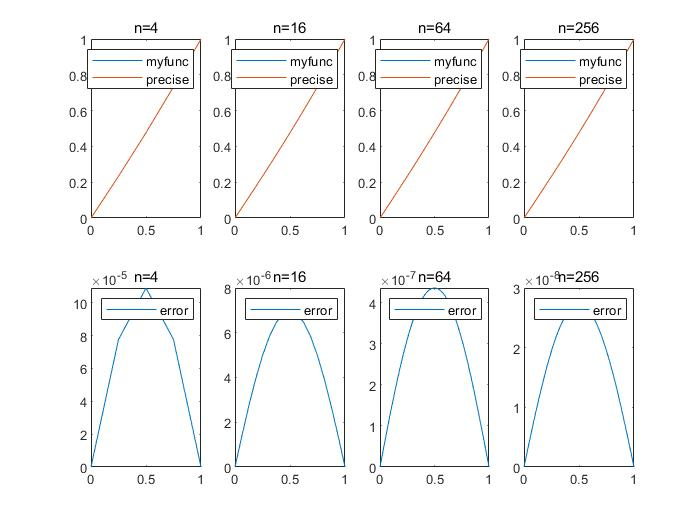
\includegraphics[width=0.6\linewidth]{result.jpg}
	}
\end{figure}
\paragraph{Q3}
The solution is visualized as follows,
\begin{figure}[H]
	\centering
	\subfigure[My result]{
		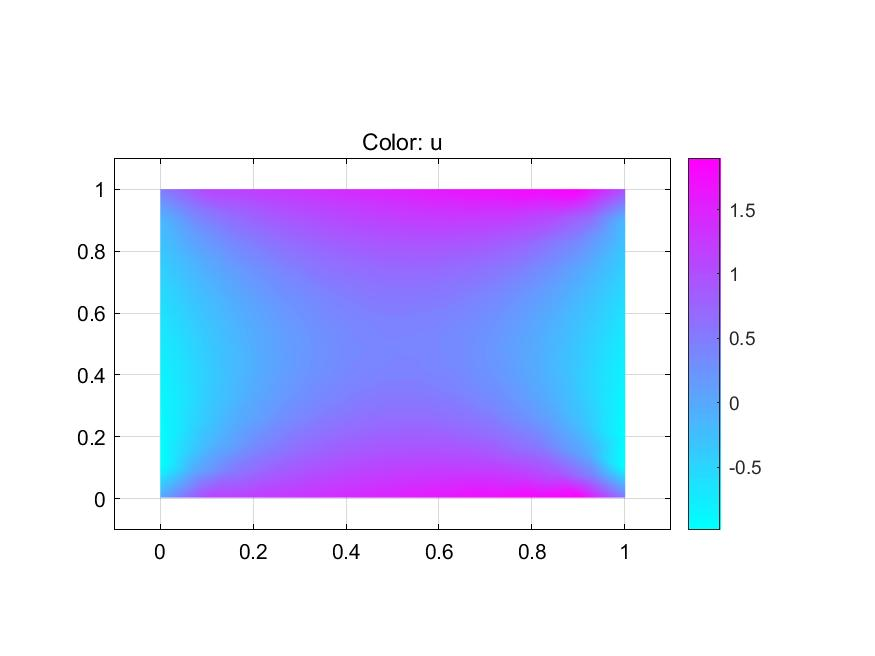
\includegraphics[width=0.6\linewidth]{2d.jpg}
	}
\end{figure}
%-------------------------------------
%=====================
\end{document}
